\documentclass{article}

% Set the margins of the page.
\usepackage[a4paper, total={6.5in, 9in}]{geometry}

% A bunch of math packages.
\usepackage{amssymb}
\usepackage{amsmath}
\usepackage{amsthm}
\usepackage{amsfonts}
\usepackage{mathtools}
\usepackage{float} % strict H figure ?

\usepackage{changepage}
\usepackage{graphicx} 		% Insert images
\usepackage{color}				% COLORS!
\usepackage[shortlabels]{enumitem}			% More enumerate types such as \alph*
\usepackage{listings}			% Used for code-blocks in latex.
\usepackage{hyperref}

% Create links when using ref and table of contents.
\hypersetup{colorlinks=true, linkcolor=black}

% Replace the indents for paragraphs with empty lines.
\usepackage[parfill]{parskip}

\usepackage[myheadings]{fancyhdr}
\usepackage{titleref}
\makeatletter
\newcommand*{\currentname}{\TR@currentTitle}
\makeatother

% Number equations with reference to sub sections.
\numberwithin{equation}{subsection}

\definecolor{lightgray}{RGB}{200, 200, 200}

% Set some style rules for code-blocks
\lstset{
	literate={<-}{$\leftarrow$}{2} {\\infty}{$\infty$}{1},
	backgroundcolor=\color{lightgray}
,
	framexleftmargin=2pt,
	framexrightmargin=2pt,
	framextopmargin=2pt,
	framexbottommargin=2pt,
	frame=single,
	basicstyle=\fontsize{10pt}{15pt}\selectfont,
	stepnumber=1,
	tabsize=4,
}


%increases table padding
\def\arraystretch{1.5}



	\title{\textbf{CSCI-2201\\Lab 2}}
\author{Anas Alhadi\\B00895875}


\begin{document}

	\maketitle
	\tableofcontents	
	\newpage

	\section{Exercise 1}
	\begin{figure}[H]
		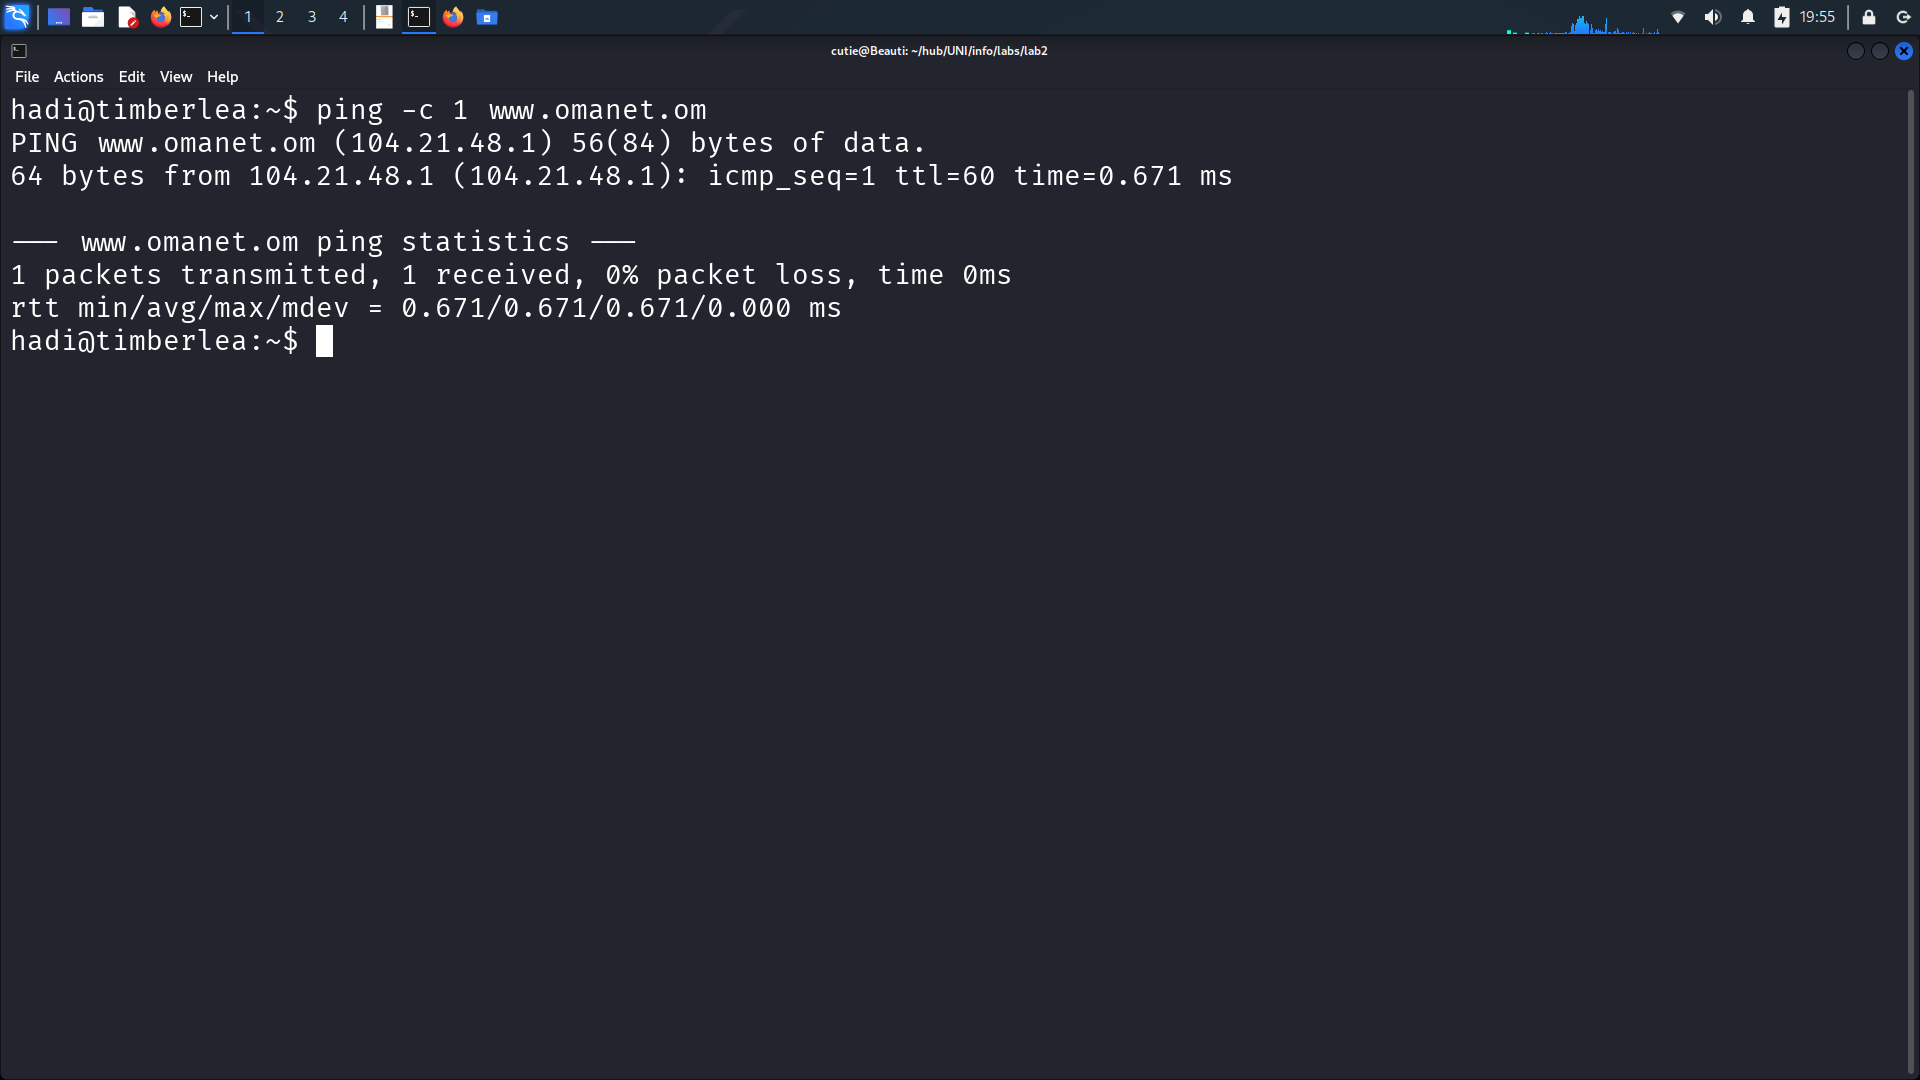
\includegraphics[width=400pt]{pics/1.png}
	\end{figure}
	\begin{figure}[H]
		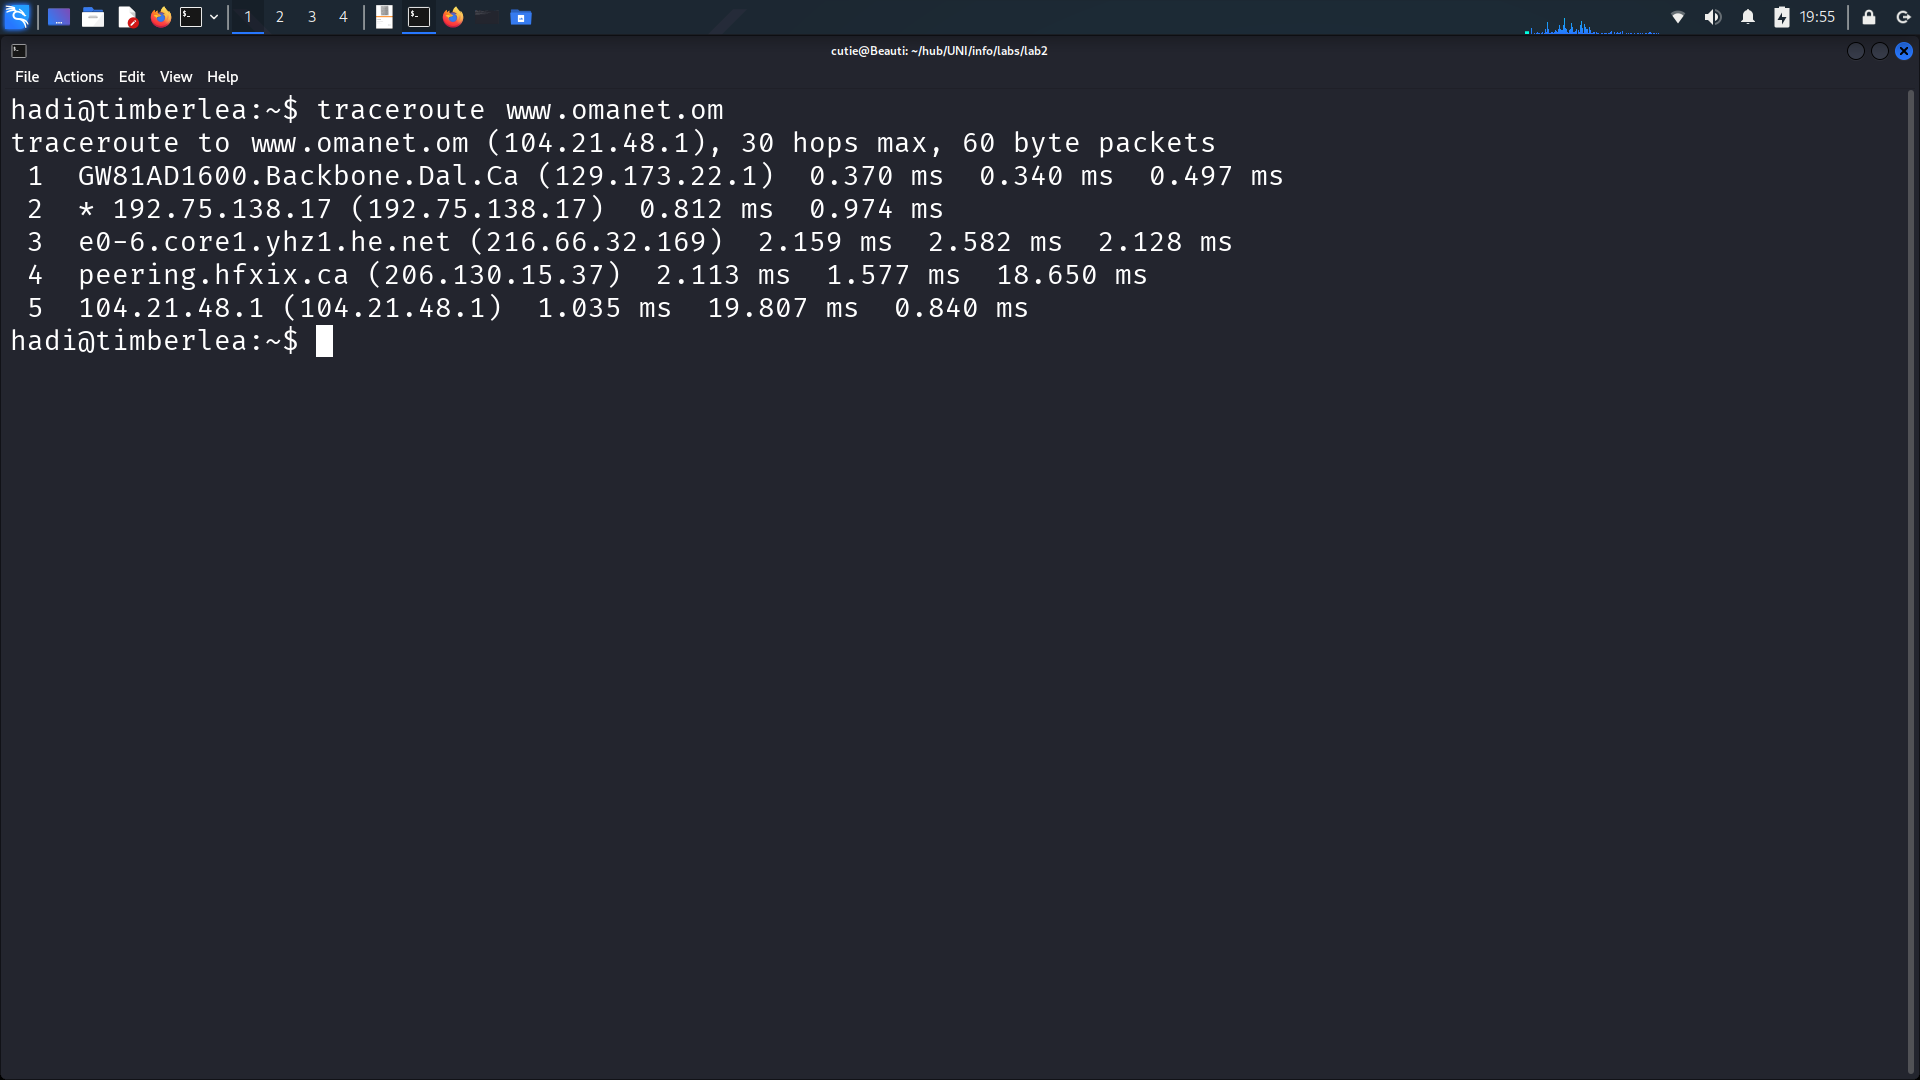
\includegraphics[width=400pt]{pics/2.png}
	\end{figure}
	\begin{figure}[H]
		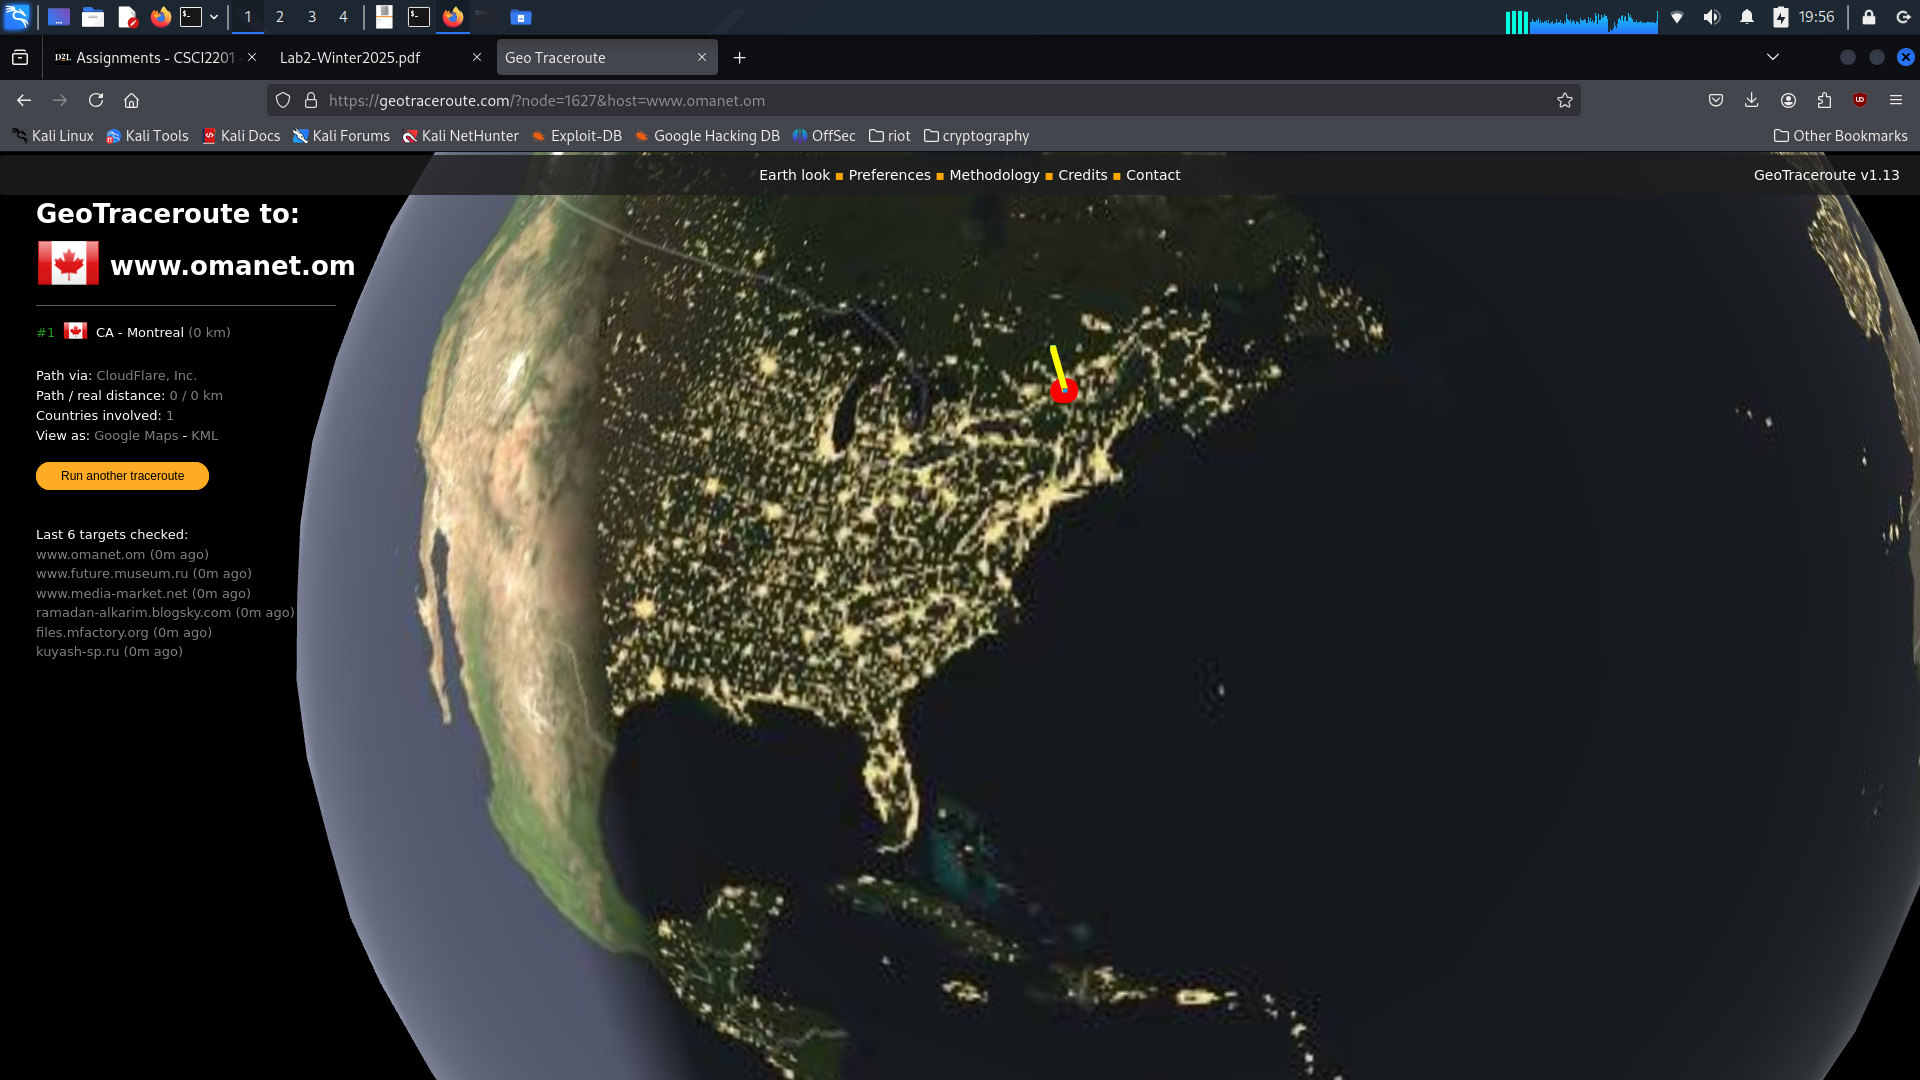
\includegraphics[width=400pt]{pics/3.png}
	\end{figure}


	\begin{adjustwidth}{1em}{1em}	
		\par{
			\textbf{Q1)} What was the first hop when tracing from timberlea, and where is the
			server located?
		}
		
		\par{
			\textbf{A)} Dal's backbone network. The server is probably in the Goldberg or
			somewhere on compus.
		}

		\vspace{10pt}
		\par{
			\textbf{Q2)} Why/why not allow pings and traceroute.
		}

		\par{
			\textbf{A)} ICMP echo requests (which are used by ping and traceroute) can be used
			to troubleshoot our servers (to check if they are up). On the otherhand, servers 
			can get ``flooded"  with echo requests (A possible vector of DDoS attacks). I think 
			servers should be allowed to respong to echo requests but also have a rate limit
			set up to stop processing such requests once we hit a specific threshold.
		}
		
	\end{adjustwidth}


	\newpage
	\section{Exercise 2}
	
	\begin{figure}[H]
		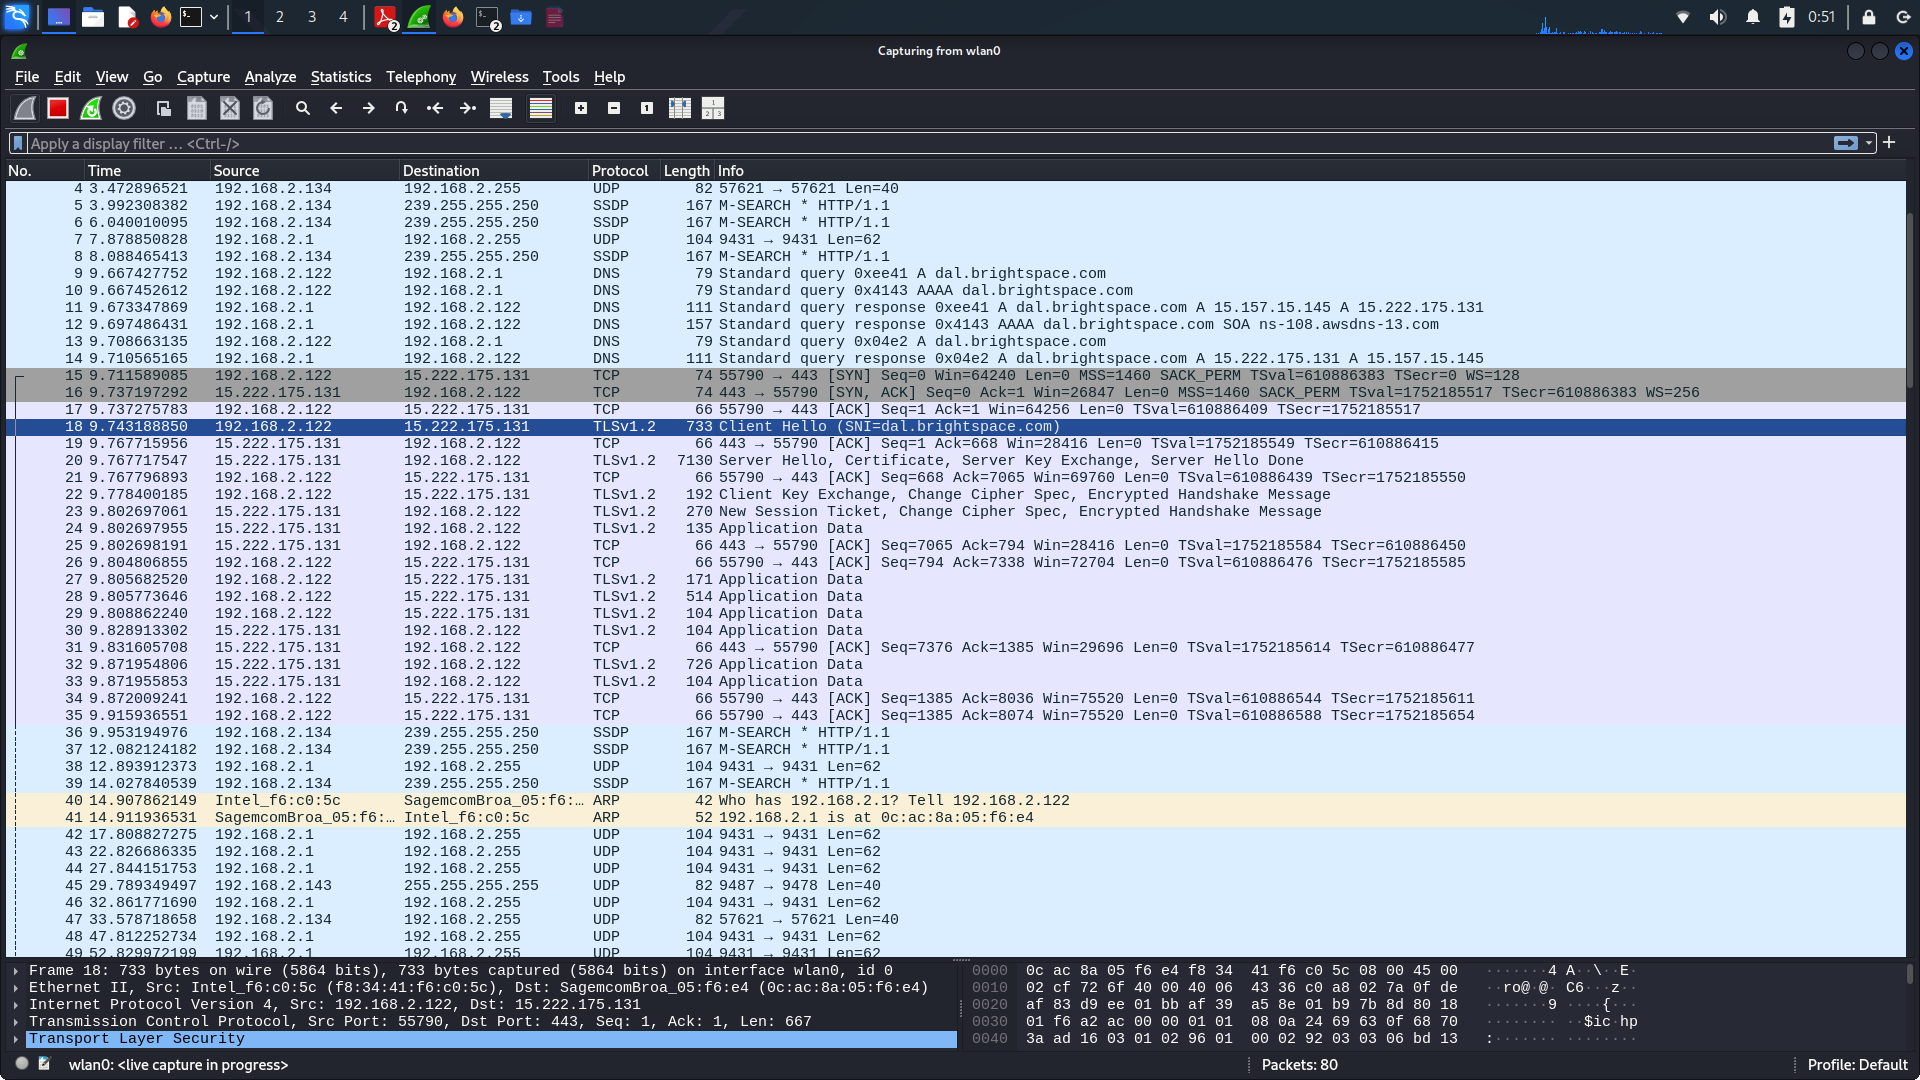
\includegraphics[width=400pt]{pics/4.png}
	\end{figure}
	
	\begin{adjustwidth}{1em}{1em}
		\par{
			\textbf{Q1)} Are there any packets
		}
		\par{
			\textbf{A)} Yes, I had firefox open in the background and also refreshed 
			the brighspace webpage.
		}
	\end{adjustwidth}

	
	\newpage
	\section{Exercise 3}
	
	\begin{figure}[H]
		\caption{Full capture}
		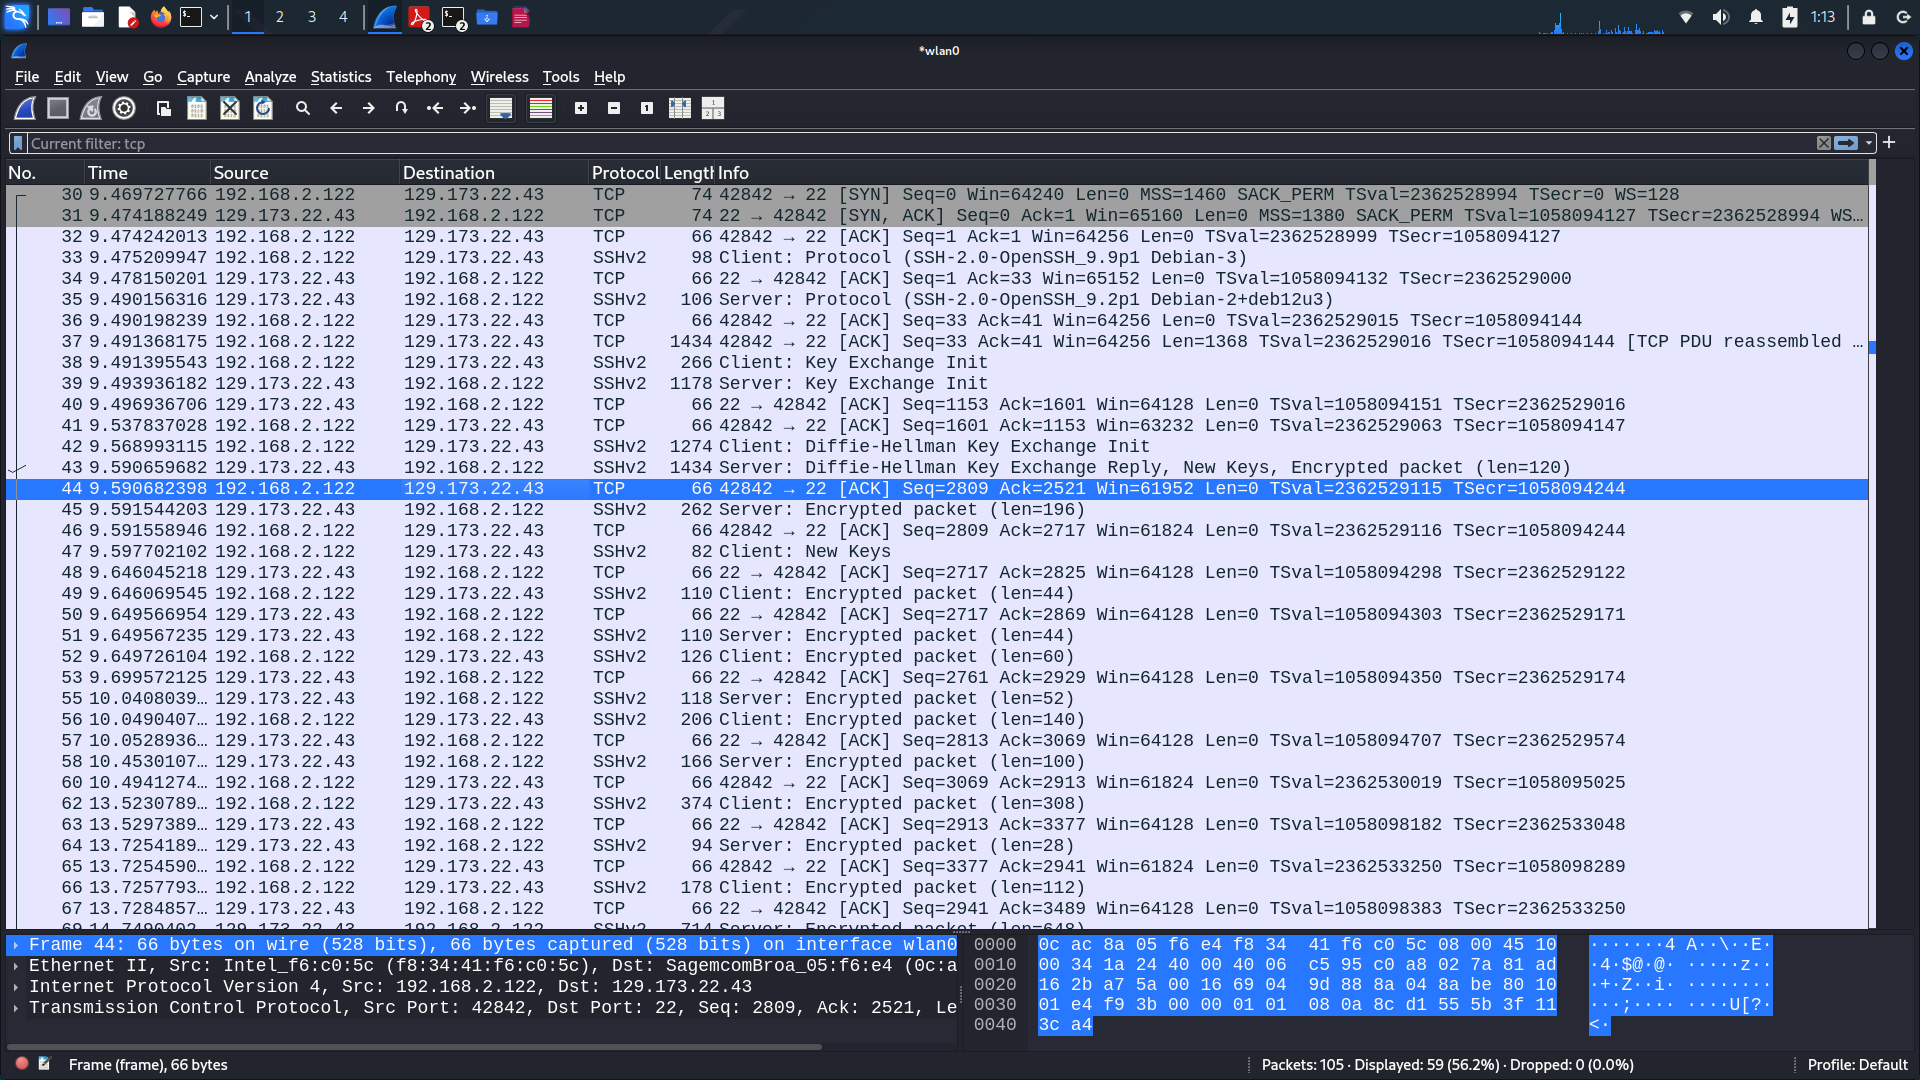
\includegraphics[width=400pt]{pics/6.png}
	\end{figure}	


	\begin{figure}[H]
		\caption{3-way handshake}
		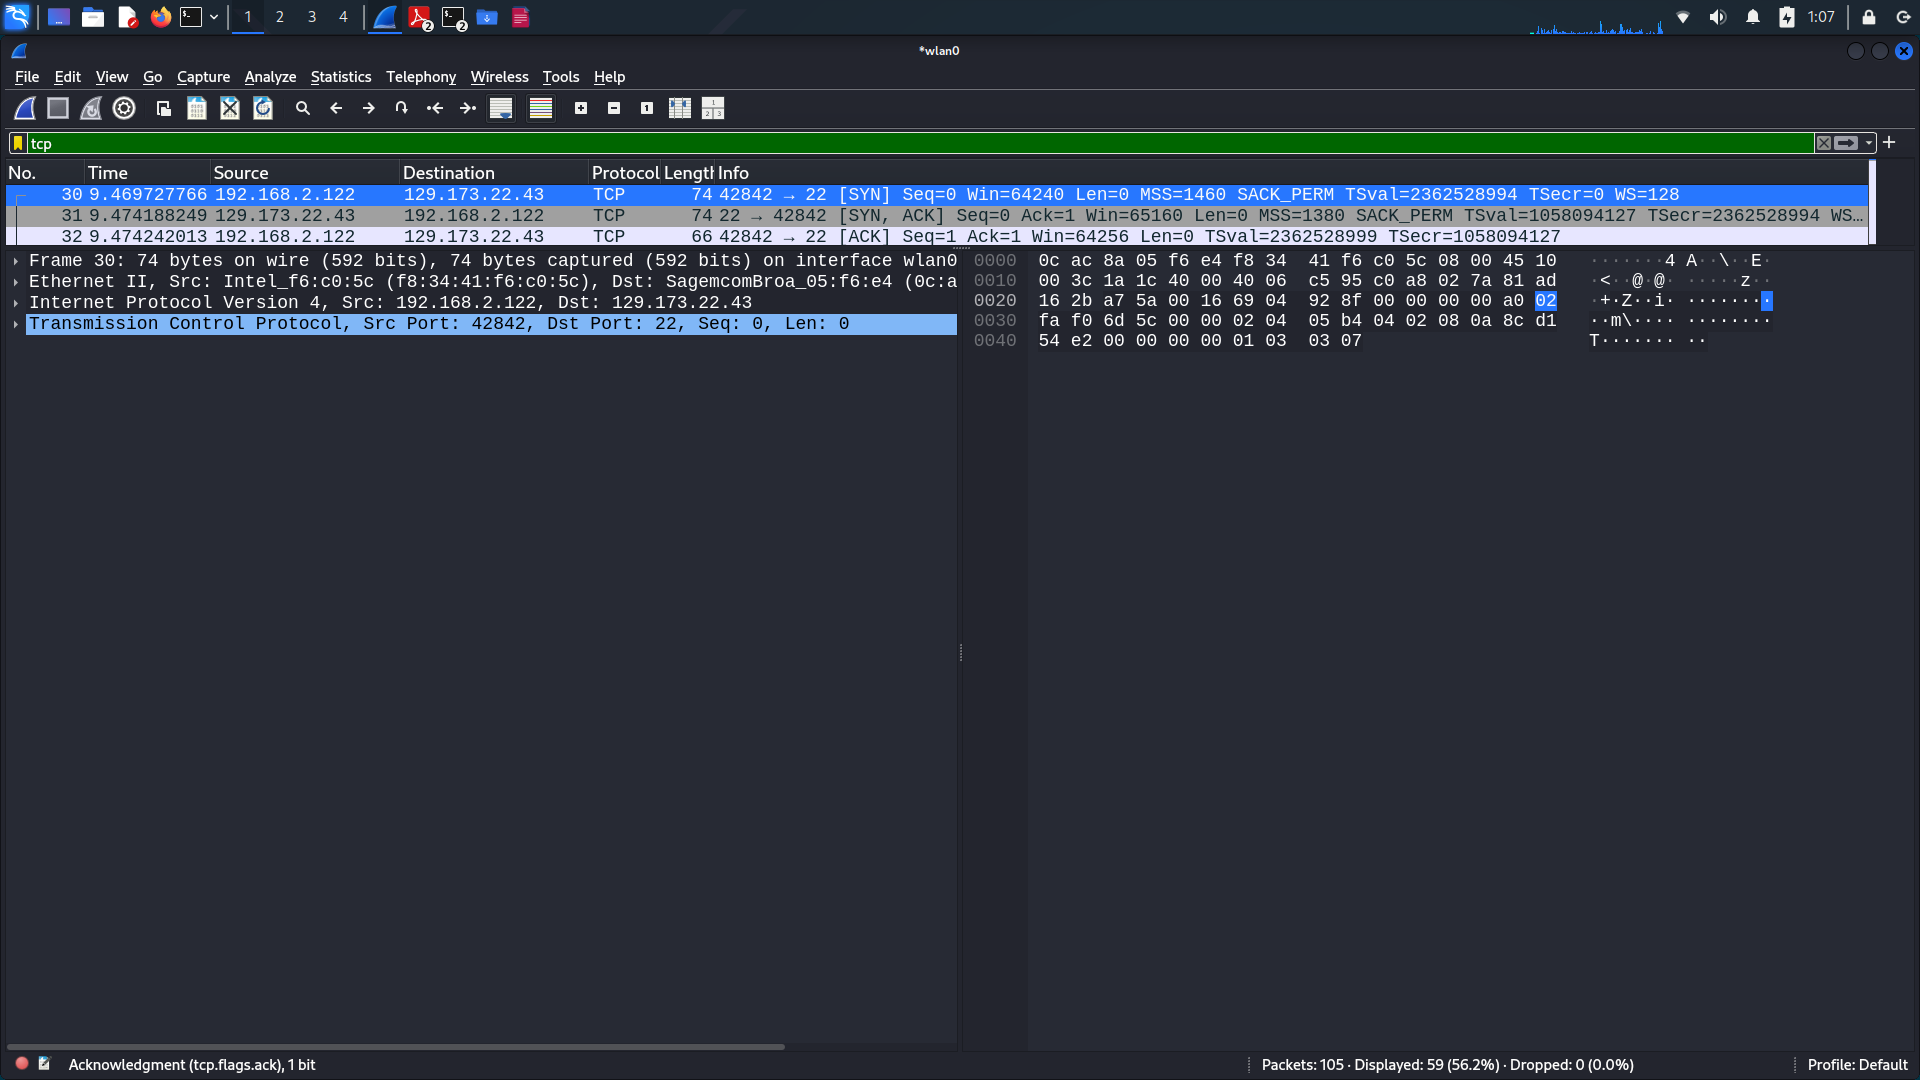
\includegraphics[width=400pt]{pics/5.png}
	\end{figure}	

	\begin{adjustwidth}{1em}{1em}
		\par{
			\textbf{Q1)} What is timberlea.cs.dal 's IP address
		}	
		\par{
			\textbf{A)}	129.173.22.43 
		}
	\vspace{10pt}
		\par{
			\textbf{Q2)} What was the port number used
		}
		\par{
			\textbf{A)} port 22, this is the standard port used for ssh.
		}
	\end{adjustwidth}

	\newpage
	\section{Exercise 4}
	\begin{itemize}
		\item \textbf{Client IP:} 192.168.4.17
		\item \textbf{Server IP:} 184.72.58.135
		\item \textbf{TLS handshake steps:}
			\begin{enumerate}
				\item Client Hello message, where it client initialtes the handshake
				\item Server Hello message, server responds with the cipher suit in our case it uses Diffie
					Helman key exchange with RSA as the authentication protocol and encrypted with AES-128
				\item Server sends is Digital Certificate
				\item Server Key exchange, server sends it's diffie helman parameters
				\item Client Key exchange, client sends it's diffie helman parameters
				\item Change Spec message, server sends a message indicating that future
					messages switch to use the key result from diffie helman.
			\end{enumerate}

		\item \textbf{Application Data:} There is no human readable data as it is now
			all encrypted after the TLS handshake.
	\end{itemize}

	\begin{figure}[H]
		\caption{Application Data}	
		\includegraphics[width=400pt]{~/Pictures/Screenshot_2025-01-31_19_57_57.png}
	\end{figure}
\end{document}
